\chapter{Microeconomic Interpretation of MATSim for Benefit-Cost Analysis}
\label{ch:economicEval}
% ##################################################################################################################

\hfill \textbf{Authors:} Benjamin Kickhöfer, Kai Nagel

\begin{center} 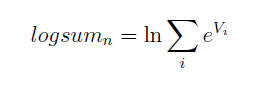
\includegraphics[width=0.25\textwidth, angle=0]{understanding/figures/logsum} \end{center}

% ##################################################################################################################

This chapter aims to explain how the agent-based framework of \acrshort{matsim} can be interpreted from a microeconomic perspective, and how it can be used for the economic evaluation of transport policies. The text of this Chapter~\ref{ch:economicEval} is an edited version of \citet[][Section~2.3]{Kickhoefer2014PhD}.

Typically, the process of economic policy evaluation consists of three steps:
%
First, forecasting the changes in the system by modeling user's reactions to a policy (Section~\ref{ch:economicEval:describingBehavior}).
%
Second, assigning some (potentially monetary) valuation to these changes (Section~\ref{ch:economicEval:valuingBehavior}).
%
And third, applying an appropriate aggregation rule (Section~\ref{ch:economicEval:aggregatingValues}).
%
As will be shown in the next sections, these steps are neither completely independent nor completely dependent on each other.

% %%%%%%%%%%%%%%%%%%%%%%%%%%%%%%%%%%%%%%%%%%%%%%%%%%%%%%%%%%%%%%%%%%%
%\vfill\eject
\section{Describing Human Behavior}
\label{ch:economicEval:describingBehavior}
Estimating benefits of a policy intervention relies on a sound descriptive model that is capable to predict the resulting behavioral changes of individuals. The following sections will therefore shortly present the concept of aggregated elasticities, followed by a presentation of Discrete Choice Theory and its relationship to the \acrshort{matsim} choice model.

%%%%%%%%%%%%%%%%%%%%%%%%%%%%%%%%%%%%%%%%%%%%
\subsection{Aggregated Elasticities}
\label{ch:economicEval:describingBehavior:elasticities}
%
%\benjamin{Kai, do we want to include elasticities in the book at all?}
%%
%\kai{finde ich passend}
%%
%\benjamin{Ok, dann lassen wir es drin.}
%
Historically, aggregated elasticities are probably the most popular concept that is used for behavioral forecasting in transport planning \citep[see, e.g.,][]{deJong2001Elasticities, 
GrahamGlaister2002FuelPriceElasticities, ParrySmall2005OptimalGasolineTax}.
%
In the simplest case, elasticities describe the change of travel demand as reaction to a monetary price change for the whole market, always relative to the status quo. Assuming an initial price level of $p_0$, a final price level of $p_1$, an initial travel demand $q_0$, and a final travel demand of $q_1$, the price elasticity of demand is defined by:
%
\begin{equation}
\eta_{q,p} = \frac{\frac{q_{1} - q_{0}}{q_{0}}}{\frac{p_{1} - p_{0}}{p_{0}}}
\end{equation}
%
That is, a relative change in the price level by $1\%$ is predicted to lead to change in travel demand of $\eta_{q,p} \%$.
%
The advantage of elasticities is that they can relatively easily be obtained from market observations, i.e.\ from measuring a change in quantities for a known price change. Instead of price changes, also changes in travel times or other behaviorally relevant parameters can be used, resulting, e.g., in travel time elasticity of demand.

However, the values depend on the particular circumstances of the measurement. Additionally, the measurement might be biased by changes in the system that occur simultaneously to the price/time changes.
%
There are many studies in the literature to determine price or travel time elasticities for mode choice, departure time choice, destination choice, travel frequency, car ownership, and activity location choice \citep[for an extensive literature review see, 
e.g.,][]{deJong2001Elasticities}. The attempt of obtaining more and more disaggregated values for single origin-destination relations, different trip purposes, income groups, etc., makes the observation very difficult, and technically leads to the estimation of individual elasticities for every person under consideration.
%
For this reason, the use of aggregated elasticities is rather inconvenient in the context of agent-based modeling where the focus is on the individual's decision making. 
%
%% These models are therefore more suitable for the use of Discrete Choice Theory in order to describe and predict human mobility behavior.
%
% Falls obiger Satz drinbleiben soll, müsste er m.E. reformuliert werden: Discrete Choice Theory is more suitable for agent-based modelling (und nicht andersherum).  Kai, oct'14

%%%%%%%%%%%%%%%%%%%%%%%%%%%%%%%%%%%%%%%%%%%%
\subsection{Discrete Choice Theory}
\label{ch:economicEval:describingBehavior:discreteChoice}
%
\benjamin{Do we want to discuss Discrete Choice Theory here, or is it already somewhere else in the book? Gunnar? The following text could be removed or moved to a section about the choice model of \acrshort{matsim}...}
%
\kai{good question.}

%% \subsubsection{Theoretical Foundations}
\label{ch:economicEval:describingBehavior:discreteChoice:foundations}
% leave that label; it should still work. kai
%
Discrete Choice Theory goes back to work by \citet{Luce1965PreferenceUtility} and \citet{McFadden1975DiscreteChoiceModel}. Two standard textbooks in this area are \citet{Ben-AkivaBook} and \citet{Train2003discreteChoiceBook}. The theory is typically used to describe individual choices among \emph{mutually exclusive} alternatives. In order to apply it to the real world, two additional preconditions need to be met \citep[p.16]{Train2003discreteChoiceBook}:
%
First, \emph{all} relevant alternatives need to be known (= choice set).
%
Second, the number of alternatives needs to be finite.
%
These alternatives need to be described by their attributes.
%
Preferences of individuals can be estimated based on survey data, which consists of different stated and/or revealed individual choices.
%
\benjamin{Some reference to the Chapter on the estimation of a utility function.}

However, the estimated parameters typically do not reproduce all individual choices correctly, or -- in other words -- individuals do not always choose the alternative with the highest utility according to their assumed utility functions; this observation violates the assumption about the consistency and transitivity of preferences. For this reason, there was a strong need for methodological improvement.
%
\citet{Luce1965PreferenceUtility} distinguished between two possible interpretations of this observed choice behavior:
%
\begin{itemize}
\item Either, people chose randomly among their alternatives (Constant Utility Model).
%
\item Or, the choice only \emph{appears} to be random, since the observer does not include all relevant decision variables in the model.
\end{itemize}
%
Since the latter interpretation is still in line with the necessary assumptions on consistency and transitivity of preferences, \citet{McFadden1975DiscreteChoiceModel} built his \gls{rum} by introducing a \emph{random component} into the utility formulation:
%
\begin{equation}
U_i = V_i + \varepsilon_i \ ,
\end{equation}
%
where $U_i$ is the utility of alternative $i$, which is \emph{perceived} by the individual; $V_i$ is the observed or systematic part of utility%
%
%described by the utility function (see Equation~\ref{XXX})%
%
%\benjamin{Some reference to the utility function of a plan}
%%
%\benjamin{I would strongly recommend to use $V_p$ instead of $U_p$ for the utility of a plan even though this is not entirely true, since some of the $\epsilon$ is already captured by the simulation noise that Gunnar called $\eta$...In consequence, the score is NOT equal to $V_p$, right?}
%%
%\benjamin{Maybe remove the \acrshort{matsim} reference here completely, and deal with the issue above in the \acrshort{matsim} section below?}
%%
%\kai{intuition to remove reference to matsim here.}
%%
%\benjamin{Agreed. Removed it, and copied my comment further down.}
%
; and $\varepsilon_i$ is a random component of utility.
%
As a result, the random component allows to chose options which do not have the highest utility with respect to $V_i$.
%% for choices that are -- according to the systematic parts of utility calculated by the utility functions -- \emph{irrational}. In consequence, there is a \emph{probability} to select the option with the highest $V_p$, as well as (lower) probabilities to select the other options with lower $V_p$. 
%
% Habe obiges mal rausgestrichen, weil man m.E. Annahmen über eps (meiner Intuition nach: Mittelwert=0) machen muss, damit die Aussage wirklich stimmt.  kai, oct'14

Assuming that all $\varepsilon_i$ are independent and identically distributed (i.i.d.)\ following a Gumbel distribution, this leads to an \gls{mnl} model with the choice probability $P_i$ for alternative $i$:
%
\begin{equation}
P_{i} = \frac{e^{\mu \cdot V_i}}{\sum_{j=1}^{J} e^{\mu \cdot V_{j}}} \ ,
\label{eq:ch:economicEval:logit}
\end{equation}
%
%% \kai{Notation für die Summe im Nenner habe ich so noch nie gesehen.  chk}
%% %
%% \benjamin{Habe es mal anders notiert. Ben-Akiva schreibt $\sum_{j \in C_n}$, wobei $C_n$ das choice set des Individuums ist. Allerdings bekommen wir mit $j$ als Index an anderen Stellen Probleme...}
%
where $J$ is the total number of alternatives in the choice set, and $\mu$ is related to the variance of the random component.%

%\footnote{
%
When estimating behavioral parameters $\hat{\beta}$ from survey data (see Section~\ref{XXX})%
%
\benjamin{Some reference to the Chapter on the estimation of a utility function.}%
%
, one actually obtains the true parameter value $\beta$ times the inverse variance of the error term distribution $\mu = \frac{1}{\sigma}$, i.e. $\hat{\beta} = \frac{\beta}{\sigma}$ \citep[see, e.g.,][p.45, where $\sigma$ is defined as \emph{scale parameter}]{Train2003discreteChoiceBook}. The scale parameter is therefore present in \emph{all} estimated behavioral parameters of the utility function.
%
%}

From the modeler's perspective, $\mu$ describes how rational (with respect to the model) decision makers behave, given a difference in the systematic part between utilities of alternatives. To give an example on the influence of $\mu$ on the choice probabilities of $J=2$ alternatives $a$ and $b$ with $V_b > V_a$: following Equation~\ref{eq:ch:economicEval:logit}, the corresponding choice probabilities are given by
%
\[
P_a = \frac{1}{1 + e^{\mu(V_b - V_a)}} \qquad P_b = \frac{1}{1 + e^{\mu(V_a - V_b)}} \qquad .
\]

%
As one can see, the choice probabilities only depend on the difference between the systematic parts of utility $V_a - V_b$,%
%
\footnote{
%
It can therefore be argued that with the use of Discrete Choice Theory, one has already left the ground of an ordinal scale of utility, since the difference in utility influences the choice probabilities.
%
}
%
and on the parameter $\mu$.
%
For $\mu \to 0$, this results in a completely random choice behavior and choice probabilities of $P_a = P_b = \frac{1}{2}$.
%
For $\mu \to \infty$, this results in a completely ``rational'' behavior and choice probabilities of $P_a = 0$ and $P_b = 1$.
%
The first case corresponds to a very large variance, the latter to a very small variance of the difference between the random components $\varepsilon_b - \varepsilon_a$.

Overall, it is important to note that individual choice behavior can again be used to calculate any desired aggregated elasticity, e.g.\ for different subpopulations.

%%%%%%%%%%%%%%%%%%%%%%%%%%%%%%%%%%%%%%%%%%%%
\subsection{Discrete Choice Theory and MATSim}
\label{ch:economicEval:describingBehavior:discreteChoice:matsim}
%
As explained in Section~\ref{sec:inbrief},
%
%\benjamin{Some reference to the loop.}%
%
agents optimize their mobility behavior over several iterations by taking the behavior of other agents into account. Even if one assumes homogeneous preferences of individuals in the behavioral parameters of their utility functions, activity locations and activity patterns of agents typically differ. In consequence, the simulation deals with heterogeneous decision makers.

Given a valid choice set for all individuals, the \acrshort{matsim} choice model is in steady state equivalent to the standard \gls{mnl} model \citep{NagelFloetteroed2009IatbrResourceInBook}.

%%%%%%%%%%%%%%%%%%%%%%%%%%%%%%%%%%%%%%%%%%%%
\subsubsection{Choice Set}
The choice set of agents can in principle be pre-computed and then be fed into the \acrshort{matsim} simulation. However, this would need to be done for every system state (e.g.\ before and after a policy change).
%
Alternatively, \acrshort{matsim} can generate choice sets of agents within the iterative loop (Section~\ref{sec:inbrief})
%
%\benjamin{Some reference to the loop.}%
%
. At the time of writing, there exist three methodological issues with the latter approach:
%
\begin{enumerate}
\item \textbf{Choice set incomplete}: The maximum number of plans $J$ in the choice set of every agent is limited by memory constraints. That is, the choice set for the decision making is unlikely to be complete.
%
\item \textbf{Plans correlation from innovation}: Plans might be correlated. This is very likely if they are modified or replaced by best-response re-planning modules (e.g.\ the route choice module), since they have a tendency to always generate the same answer. Yet also random mutations in general result in correlated plans, since the concept of a mutation in fact implies an only small change away from the parent.  This violates the required IIA (Independence from Irrelevant Alternatives) 
% _from_ !!
property of the choice set that is needed for an \gls{mnl} 
% _an_ eMeNel !!
model.\footnote{%
%
A possible approach to increase the diversity in route choice is investigated by \citet{NagelKickhoeferJoubert2014HeterogeneousVoTsPROCEDIA}.
%
}

\item \textbf{Plans correlation from plans removal}: The current \acrshort{matsim} implementation has a tendency to keep similar, i.e.\  correlated, plans when the number of plans has grown beyond $P$.  The reason for this is that the current plans remover removes the plan with the lowest score, which typically also is the one most different from the other plans.  As a result, typically only very similar plans with very similar scores remain in the choice set.\footnote{%
%
A possible approach to maintain diversity in plans removal would be to give penalties to the scores of plans that are similar to other plans.  This penalty could be taken directly from approaches such as the path size logit \citep{DaganzoSheffi1977SUE,FrejingerBierlaire2007PathSizeLogit}.  For early attempts within \acrshort{matsim} see \cite{Grether2014PhD} (Chapter~6) and \cite{NeumannEtAlPassengerArrivalPatterns}.
%
}


\end{enumerate}
%
These three issues might lead to biased behavior, and also have consequences for economic evaluation. A discussion of these aspects, as well as a presentation of possible solutions will be given in the upcoming sections.

%%%%%%%%%%%%%%%%%%%%%%%%%%%%%%%%%%%%%%%%%%%%
\subsubsection{Randomness and Self-consistent State}
\label{ch:economicEval:describingBehavior:discreteChoice:quenchedVsAnnealed}
%
\kai{Folgendes müsste eigentlich bereits weiter oben im Buch drin stehen.}
%
\acrshort{matsim}, as a simulation engine that uses random numbers, produces randomness.
%%
%% The process from one iteration to the next is Markovian.\footnote{%
%%
%% Typically, an iteration only uses the events from the last iteration, and the plans. As long as the system does not keep an infinite memory, there is always a way to make the memory of the system part of its state.
%%
%% }
%
A straightforward interpretation is obtained when one assumes that both, the choice set and the score $S_{n,i}$ of each plan, 
%% individual scores of person $j$ for plan $p$, $S_{j,p}$,
%
%% \benjamin{Chk indices!}
%
are fixed.Then in each iteration each agent makes a draw from its choice set according to its scores, based on the choice model(s) defined in the configuration file (see Section~\ref{sec:config}).
%\footnote{%
%
%\kai{Some pointer to the config file chapter.}
%
%}
%
That is, under these conditions \acrshort{matsim} becomes a Monte Carlo engine
%
(see Chapter~\ref{ch:monteCarlo})
%\footnote{%
%
%\benjamin{Some pointer to the Monte Carlo chapter.}
%
%}
%
that samples from the choice sets and then computes a (stochastic) realization of the network loading based these choices.

Under these conditions, a self-consistent solution is reached when each plan's score $S_{n,i}$ corresponds to the expectation value of that plan's performance under these conditions.
%
%% $E(U_{n,i}) = S_{n,i} + E(\eta_{n,i}) + \epsilon_{n,i}$, 
%% %
%% \benjamin{Is this correct? Would need to define $\eta$}
%
%given that all other plans of all other agents are treated the same way.
%
This is conceptually similar to the \gls{sue} behavior \citep{DaganzoSheffi1977SUE}, but interprets the \gls{sue} as true repeated random draws instead of deterministic flow fractions \citep{NagelFloetteroed2009IatbrResourceInBook}.

Such behavior can be approximated
%
%% \benjamin{How much of an approximation is that?}
%
in \acrshort{matsim} by
%
\begin{itemize}
\item setting the configuration option \verb$fractionOfIterationsToDisableInnovation$ below one,  meaning that for the remaining fraction of iterations innovation will be switched off, i.e.\ the choice sets will remain fixed from then on;

\item setting the configuration option \verb$fractionOfIterationsToStartScoreMSA$ below one, meaning that for the remaining fraction of iterations scores will be averaged according to the \gls{msa}.\footnote{%
%
An even better approach, potentially to be implemented and investigated in the future, would be to actively check for convergence and stop when it has been sufficiently achieved.
%
}
\end{itemize}
For the remainder of this Chapter \ref{ch:economicEval}, it will be assumed that such a self-consistent solution has been found.
%% at some iteration the choice set was fixed, and the score has afterwards self-consistently converged in this way.
%% in the way that the expectation value of the choice behavior/network loading based on those scores replicates exactly those scores.
%
%% \benjamin{I find that hard to translate in the sense of ``how do I as a user know whether the above conditions are given for my simulation'' -- maybe add some more intuitive explanation?}
%% %
%% \benjamin{Especially, what is ``self-consistent convergation'', ``expectation value'', ``replicates those (which?) scores''?}
%% %
%% \kai{Habe jetzt einfach ``such a self-consistent solution has emerged'' geschrieben.  Klärt es das?  Ansonsten: Es ist die SUE-Definition; vielleicht kannst Du es besser ausdrücken?}

%% A remaining problem is that some of the variance that in a \gls{RUM} is parameterized by the random component $\epsilon_i$ in \acrshort{matsim} is modelled explicitly.
%% explicitly considered in the traffic flow simulation/network loading.
%
%% \benjamin{Do we want to use traffic flow simulation or network loading?}

A remaining issue then is that the randomness that is explicitly contained in MATSim needs to be consistent with the discrete choice model.\footnote{
%
\benjamin{Some pointer to Gunnar's chapter where it is discussed under what conditions $S_{n,i} = V_{n,i}$ or $S_{n,i} = U_{n,i}$ or something completely else.}
%
}
%
For example, the propensity to use public transit might depend on the distance to the next transit stop, or how well that stop connects to the destination to which the person is traveling.  \acrshort{matsim} will pick up such effects explicitly.  Only a choice model which considers the same attributes will be consistent; otherwise, some of the above effect will be considered as random from the point of view of the analyst and thus be moved into the $\varepsilon_i$, and subsequently into the scale parameter $\mu$.
%
%% \benjamin{Based on that: what do we recommend in the following section? Logsum, executed, or average? I read it as if we should recommend using the executed plan's score, but then we need to write it somewhere...}
%
% nope. if anything, then this points to logsum term.  But so far it only talks about self-constent solition. kai
%
%% This, in consequence, means that $\sigma$  in the \gls{mnl} model is greater than in \acrshort{matsim}, and the resulting $\beta_X$
%% %
%% \kai{index?}
%% %
%% from the estimation are smaller than what would be correct inside \acrshort{matsim}.
%
%given that these effects are already absorbed.
%
%% \benjamin{Removed the last part of the last sentence since in my opinion it confuses more than it helps. Also adjusted the text above. @Kai: can you check whether you are ok with that?}
%
%ok. kai, oct'14

%%%%%%%%%%%%%%%%%%%%%%%%%%%%%%%%%%%%%%%%%%%%
\subsubsection{Frozen Randomness}
\label{sec:frozen-randomness}
%
\kai{auch das jetzt folgende sollte schon woanders im Buch sein!} \ah{Chapter~\ref{ch:destinationchoice}. Zitierweise in diesem Abschnitt verbesserungsbedürftig.}.
%
The interpretation in Section~\ref{ch:economicEval:describingBehavior:discreteChoice:quenchedVsAnnealed} assumes that each \acrshort{matsim} agent performs repeated random draws according to its choice set and its choice model. 
%
In other words:
%
\begin{itemize}
\item It is assumed that the scores $S_{n,i}$ have converged and correspond to the systematic parts of utility $V_{n,i}$. In consequence, also the choice probabilities $P_{n,i}$ have converged.
%
\item However, making repeated random draws from these probabilities effectively \emph{parametrizes} the effect of randomly re-drawing the $\varepsilon_{n,i}$, and then taking the option $i$ where $U_{n,i} = V_{n,i} + \varepsilon_{n,i}$ is maximal. That is, the alternative with the highest utility might vary.
\end{itemize}
%
%% %
%% In other words, although the scores
%% %
%% \kai{$= V$}
%% %
%% themselves have converged, one can imagine that the $\varepsilon_i$ are randomly re-drawn every time the agent makes a new choice.
%% %
%% \benjamin{I would add: ``...because of the variation produced by the \acrshort{matsim} traffic flow simulation.''}
%% %
%% \benjamin{Wobei: das macht eigentlich keinen Sinn; aber inwiefern werden die epsilons denn re-drawn?}
%% %

An alternative approach is to ``freeze'' the epsilons directly into the plans.  \kai{nicht komplett identisch mit Horni, aber ähnlich!!}  In this interpretation, each plan $i$ would obtain a fixed $\varepsilon_{n,i}$ at construction, which would only change when the plan changes.  In consequence, once the choice set becomes fixed, also each plan's $\varepsilon_{n,i}$ would become fixed, and the choice model should then deterministically select the plan with the highest score \emph{including the plan's $\varepsilon_{n,i}$}.
%
%% $\benjamin{I would add: ``That is, the score $S_{n,i}$ would be interpreted as $U_{n,i}$ from the estimated \gls{mnl} model.''}
That is, the score $S_{n,i}$ would be directly interpreted as the total utility $U_{n,i}$.
%
Such an approach can currently not be configured for \acrshort{matsim}; it needs to be programmed explicitly in Java. This has been performed for destination choice (see Chapter~\ref{ch:destinationchoice}) \ah{Typisches Beispiel für Genetic Drift. Frozen-Randomness und eine Methode das auch berechenbar zu machen wurde für Locationchoice nicht einfach bloss angewendet, sondern erfunden. }.

Such an approach seems to be quite commonly used for project evaluation with discrete choice models \kai{look into the ahorni paper}.  The models do not compute these frozen $\varepsilon_i$ explicitly.  Yet, they are started both for the base case and the policy case with the same random seed, which means that effectively in each choice the random numbers are the same between base and policy case.  A different choice in the policy case can thus only occur when the systematic utilities change.

%% As an approximation, one can assume that the $\varepsilon_i$ for plans with different routes, modes and times are zero.
%% %
%% %% \benjamin{I would add: ``That would imply that the variation produced by \acrshort{matsim} is assumed to be equal to the $\varepsilon_i$ in the estimated \gls{mnl} model, i.e.\ that the score $S_{n,i}$, again, can be interpreted as $U_{n,i}$ from the estimated model.''?}
%% %
%% Recall that for the present chapter we assume that all scores are converged, i.e.\ we are looking at their expectation values.  This is straightforward to configure in \acrshort{matsim} by using the \verb$BestScore$ module for plan selection, but it is unclear how to estimate the necessary utility function.

%% \kai{Benjamin, meine Intuition ist, dass das nicht anders geht: Wenn wir das als Option drinhaben wollen, dann muss dies irgendwo rein.  Es könnte höchstens unter ``outlook'', dann wäre also die logsum interpretation der derzeitige Weg, und dies hier wäre eine zukünftige Möglichkeit.  --  Vielleicht besser, aber jetzt habe ich es erstmal an dieser Stelle hier getippt.}

%% \benjamin{Finde ich ok. Können wir am Ende immer noch in den Outlook schieben.}


% %%%%%%%%%%%%%%%%%%%%%%%%%%%%%%%%%%%%%%%%%%%%%%%%%%%%%%%%%%%%%%%%%%%
%\cleardoublepage
\section{Valuing Human Behavior at the Individual Level}
\label{ch:economicEval:valuingBehavior}
Following \citet{deJongEtAl2007LogsumTRA}, a major advantage of the agent-based approach is that it allows for a seamless integration of (i) forecasting behavioral changes as a reaction to changes in the system, and (ii) the subsequent economic evaluation.
%
In this section, it is shown how estimated agent-specific preferences which determine behavior can directly be used for deriving individual \glspl{vtts}, and how they need to be modified for running a \acrshort{matsim} simulation in order to obtain individual utility differences resulting from a policy.
%
The subsequent Section~\ref{ch:economicEval:aggregatingValues} will then focus on how these individual utility changes can be used in order to derive some indicator of overall welfare change for the population under consideration.

%%%%%%%%%%%%%%%%%%%%%%%%%%%%%%%%%%%%%%%%%%%%
\subsection{The Utility of Time}
\label{sec:scor-funct-revisited}
The \acrshort{matsim} scoring function of plan (= alternative) $i$ consisting of $q = 1..Q$ activities and trips has been introduced in Chapter~\ref{???} in the following form:\
%% footnote{\label{footnote:income-effects}%
%% %
%% The approach is motivated by \citep{Small2012ValuationOfTimeRevisited}; similar arguments are made, e.g., by \citep{DeSerpa1997economicsOfTime, JaraDiaz2003TimeAllocationTheory, Jara-DiazGuevara-2003}.  The term related to the marginal wage rate is removed, since this is currently not considered in \acrshort{matsim}.  In consequence, the utility of gaining or losing money is moved into the direct utility function.  The linear formulation implies that income effects \citep{HerrigesKling1999Nonlinearincomeeffects,DalyEtAl2008WelfareMeasuresIncome, DagsvikKarlstrom2005ChoiceProbabilitiesInNonlinearRUM,Jara-Diaz1989IncomeEffectsInModeChoice} are currently not considered, i.e.\ the monetary effect of any change is not strong enough to change $\lambda$.
%% %
%% }
%% \footnote{%
%% %
%% The mode-specific notation is omitted here for clarity reasons.  \kai{Sehe gar nicht, warum diese Fußnote nötig ist.  Jeder ``trip'' hat hier doch einen separaten Index $q$, somit auch ein anderes $\beta_q$, und unter welchen Voraussetzungen die evtl.\ identisch sein können (weil sie z.B.\ vom selben mode kommen), wird gar nicht diskutiert.}
%% %
%% }
\begin{equation}
U = \sum_q U_{act,q}(t_{dur,q}, ...) + \sum_q U_{trav,q}(t_{trav,q}, ...) 
%
%+ \lambda \cdot (Y - G) 
\ ,
\label{eq:scoring-fct-revisited}
\end{equation}
%% where $Y$ is ``unearned income'' \citep{Small2012ValuationOfTimeRevisited} (for example a possible toll refund) and $G$ are payments, for example tolls or fares.
where monetary payments (e.g.\ tolls) are included into $U_{trav,q}$ and the index $i$ was dropped for notational convenience.


An approximate argument about optimal time allocation can be made as follows.
Assume the constraint
%% \footnote{%
%% %
%% The following is derived from \citep{Small2012ValuationOfTimeRevisited}; similar arguments are made, e.g., by \citep{DeSerpa1997economicsOfTime, JaraDiaz2003TimeAllocationTheory, Jara-DiazGuevara-2003}.  The term related to the marginal wage rate is removed, since this is currently not considered in \acrshort{matsim}.  This makes it, in fact, questionable if the monetary term should be kept as a constraint, or rather included into the direct utility.  As long as one assumes that the conversion of money into utility is linear, there is no immediate difference between these two approaches.  \kai{Wäre es besser, ein $U_{money}$ in die direkte Nutzenfunktion einzubauen?  Die Small'sche Eleganz, dass VoT eine Division zweiter Langrange-Parameter ist, haben wir ohnehin bereits eingebüsst.}
%% %
%% }
%% %
%% \begin{itemize}
%% \item 
$T - \sum_q t_{dur,q} - \sum_q t_{trav,q} = 0$, i.e.\ that the time per day is limited by $T = 24h$, during which all trips and activities need to be completed.
%% \item $Y - G \ge 0$. $Y$ is unearned income, for example from a toll redistribution; $G$ is payments, for example tolls or fares.
%% \item $T_{trav,q} - t_{trav,q} \le 0$.  This states that there is some minimum mode-specific travel time $T_{trav,q}$ that cannot be reduced any more for trip $q$.  In general, this constraint is binding, since no additional utility can be derived by traveling longer than $T_{trav,q}$.
%
%% \benjamin{This constraint could be moved direcly into $U_{trav,q}$.}
%
%% \end{itemize}
%
Let us for now also assume that all travel times are fixed, i.e.\ we ignore the possible optimization that can come from departure time or mode switches, and let us thus concentrate on the activity time allocation problem.
%
Optimizing under 
%these constraints 
this constraint leads to the Lagrangian
\begin{equation}
L = \sum_q U_{act,q}(t_{dur,q}, ...) + \sum_q U_{trav,q}(t_{trav,q}, ...)
%
%+ \lambda \cdot (Y - G)
%
+ \mu \cdot (T - \sum_q t_{dur,q} - \sum_q t_{trav,q})  \ .
\label{eq:lagrangian}
\end{equation}
%% \[
%% - \sum_j \phi_j \cdot (T_{trav,j} - t_j) \ ,
%% \]
%% where the last constraint is added with a negative sign since more minimum time for travel typically leads to a lower utility (i.e.\ we want $\phi_j$ positive).

%% For solving the optimization problem, one has to note that in the above formulation only the $t_{dur,q}$ can be modified by the agent.  \kai{what about paying more for a faster train?}  
Solving the optimization problem leads to
\begin{eqnarray}
%% 0 & \stackrel!= & \frac{\partial L}{\partial t_j} = U'_{trav,j}(t_j) - \mu + \phi_j \label{eq:trav} \\
%% %% 0 & \stackrel!= & \frac{\partial L}{\partial t_w} = U'_{act,w} - \mu + \lambda \, w 
%% %% \label{eq:work} \\
0 & \stackrel!= & \frac{\partial L}{\partial t_{dur,q}} = U'_{act,q}(t_{dur,q},...) - \mu 
%
\qquad (\forall q)
\label{eq:acts}
\end{eqnarray}
and the time constraint equation from above.
%
%% Inserting Equation~(\ref{eq:trav}) into (\ref{eq:vot}) leads to
%% \[
%% VoT = - \frac{U'_{trav,j}}{\lambda} + \frac{\mu}{\lambda} \ .
%% \]
Equation~(\ref{eq:acts}) states that, at the optimum and without further constraints%
%
%% \footnote{%
%% %
%% For a discussion on the influence of further constraints (e.g.\ opening times, income), please see Section~\ref{???}.
%% %
%% }%
%
, the $t_{dur,q}$ need be selected for all activities $q$ such that all $U'_{dur,q}(t_{dur,q},...)$ are the same and equal to $\mu$.

Equation~(\ref{eq:lagrangian}) can also be seen as a linearized version of the indirect utility function
%
\kai{gibt es dafür eine Referenz?}%
%
\benjamin{Habe gesucht, aber keine gefunden...ggf. hier \url{http://eml.berkeley.edu/~webfac/saez/e131_s04/taxes.pdf}: ``the derivative of the indirect utility function should equal the Lagrange multiplier on the budget constraint''; Ist halt Lehrbuchwissen...}%
%
; for example, reducing the duration of travel by $\Delta t_q$ does not only affect $U_{trav,q}$ but will also lead to a utility change of $ \mu \cdot \Delta t_q$ from the constraint, which can be interpreted as the linearized utility effect of spending that time otherwise.
%
In consequence, the \textbf{marginal utility of time spent traveling} reads
%
\begin{equation}
\frac{\partial L}{\partial t_{trav,q}} = U'_{trav,q}(t_{trav,q},...) - \mu \ .
\label{eq:marg-UoT}
\end{equation}
%
$\mu$ is the \textbf{marginal utility of time as a resource} -- the marginal utility generated by increasing $T$, i.e.\ by making the day longer than 24~hours.
%
The marginal utility of time spent traveling is thus determined by $\mu$, modified by ``any enjoyment or dislike of the travel itself'' \citep{Small2012ValuationOfTimeRevisited}.

In order to get a handle onto the \acrshort{matsim} utility function in Equation~(\ref{eq:scoring-fct-revisited}), $\mu$ and $U'_{trav,q}$ need to be obtained separately -- $\mu$ in order to calibrate $U'_{act,q}$ as in Equation~(\ref{eq:acts}), and $U'_{trav,q}$ in order to calibrate the \emph{direct} utility of traveling, which now is an ``offset'' to the marginal utility of time as a resource.
%
This will be further discussed in Section~\ref{ch:economicEval:valuingBehavior:estimates2Matsim}.


%%%%%%%%%%%%%%%%%%%%%%%%%%%%%%%%%%%%%%%%%%%%
\subsection{The Utility of Money}
\label{ch:economicEval:valuingBehavior:uom}
Typical time allocation theory \citep{DeSerpa1997economicsOfTime, Jara-DiazGuevara-2003} makes a similar argument for money, with a budget constraint similar to the time constraint.
%
In the same way as the time constraint leads to a marginal utility of time as a resource, the budget constraint leads to a marginal utility of money as a resource.

However, \acrshort{matsim} does not include such a monetary budget constraint. It is also questionable if one should introduce it: The typical theoretical argument assumes the possibility to increase one's income by working more hours, and it is questionable if this is applicable to European countries where work contracts typically include a fixed number of working hours which cannot easily be changed.  
%% the typical derivation holds for European countries, since that typical derivation assumes that there one can increase one's income by working more hours.
%% where work contracts typically include a fixed number of working hours.  
%
Hence, an alternative derivation of the marginal utility of money needs to be found.

Assume that $U_{trav,q}$ includes a monetary component $- \lambda \, c$.  Then
\[
%\frac{\partial L}{\partial c} =
%
\frac{\partial U}{\partial c} 
%
= \frac{\partial U_{trav,q}}{\partial c}
%
= - \lambda \ ,
\]
that is, increasing a cost by $\Delta c$ reduces the utility by $- \lambda \cdot \Delta c$.
%
We will interpret $\lambda$ as the \textbf{marginal utility of money}.%
%
\footnote{\label{footnote:income-effects}
%
This constant, potentially person-specific factor, implies that income effects \citep{HerrigesKling1999Nonlinearincomeeffects,DalyEtAl2008WelfareMeasuresIncome, DagsvikKarlstrom2005ChoiceProbabilitiesInNonlinearRUM,Jara-Diaz1989IncomeEffectsInModeChoice} do not play a role, i.e.\ that changes in monetary expenses resulting from transport policies are not strong enough to change $\lambda$.
%
}

%
Note that taking the first derivative of $L$ with respect to $c$ would lead to the same result.

That is, other than for the utility of time above, we do \emph{not} decompose the  marginal utility of spending money for travel into a marginal utility of money as a resource plus an ``offset'' for spending money on that particular purpose.  The reason for this is that, since there is no (budget) constraint, there is also no ``neutral'' Lagrange multiplier that would give the marginal utility of money as a resource.

This, however, leads to the problem that if there are multiple monetary channels, they may have different marginal utilities of money.  For example, it commonly found that the marginal utility of toll payments is larger than the marginal utility of payments for fuel -- i.e.\ people find it less irritating to pay for fuel than to pay toll 
%
%\kai{Benjamin, hättest Du eine citation hierfür?}%
%
\citep[see, e.g.,][]{VrticEtc2008ReisekostenSVIBericht}.
%
%% In the original theory, the marginal utility of money, $\lambda_n$, is a Lagrange multiplier.  \cite{Small2012ValuationOfTimeRevisited} points out that it is difficult to estimate; for example, it is \emph{not} the marginal utility of income.  In the formulation of Equation~(\ref{eq:scoring-fct-revisited}), it is instead included into the direct utility.  This makes it seemingly a bit easier, but the problem remains the same: 
That is, each monetary channel, such as petrol cost, toll, public transport fare, or a 
toll refund, may lead to a different pre-factor in estimation.

To our knowledge, there is no best solution to this problem in the literature.  For the time being, we work with forcing all cost-related parameters of all alternatives to the same value in preference estimation.
%%  as it was done in Equation~(\ref{eq:ch:economicEval:utilityTraveling}).%
%% %
%% \footnote{
%% %
%% To the knowledge of the authors, there is no best solution to this problem in the literature. The single value for the marginal utility of money is rather a necessary convention.
%% %
%% }
%
However, choice modelers typically avoid to limit the model's degrees of freedom since it suppresses some information contained in the data.\footnote{%
%
J. de Dios Ort\'uzar, personal communication.
%
}
%
It is therefore often not possible to obtain the necessary parameter estimates from the literature. Where the raw data is available, the same model can be re-estimated with a uniform marginal utility of money across alternatives
\citep[see, e.g.,][]{KickhoeferEtAl2011PolicyEvaluationIncome, TirachiniEtAl2012CrowdingCongestion}.

Also, \cite{Small2012ValuationOfTimeRevisited} points out that the ``neutral'' marginal utility of money as a resource is difficult to estimate; for example, it is \emph{not} the marginal utility of income.  As an alternative research avenue, we can imagine that the monetary channels of a measure are included into the choice experiment.  For example, a travel time improvement in a value-of-time study could come together with a hypothetical income tax increase \emph{or} with a hypothetical toll.  A rudimentary version of this actually takes place in Switzerland, where large infrastructure investments are bundled with tax increases that pay for them before they are put to public vote. \kai{citations?}

%% \kai{Man könnte hier einwerfen, dass man es sonst wie bei der Zeit machen sollte: Wähle einen Zahlungskanal für die ``marginal utility of money as a resource'', und gib' alle anderen relativ dazu an.  Auch hier: haben wir bisher nicht gemacht. }

%% Note that even a model with a uniform marginal utility of money may still have mode-dependent\gls{vtts}, since the $\hat{\beta}_{tr}$ may still be mode-dependent.




%% Sec.~\ref{ch:economicEval:aggregatingValues:discussion:muom} discusses alternatives in order to obtain this value.

%%%%%%%%%%%%%%%%%%%%%%%%%%%%%%%%%%%%%%%%%%%%
\subsection{Value of Time}
%% Under the above assumptions, $\mu/\lambda$ is the \textbf{resource value of time}.  $(\mu/\lambda) \cdot \delta$ is the willingness to pay for a (theoretical) extension of the day beyond $T$ by $\delta$.

The \textbf{\gls{vtts} of trip $q$} is defined as
%
\begin{equation}
VTTS_q = \frac{\partial L/\partial t_{trav,q}}{\partial L/\partial c} \ ,
%% = - \frac{U'_{trav,q}}{\lambda} + \frac{\mu}{\lambda} \ ,
\label{eq:vot}
\end{equation}
%% that is, the marginal change of the indirect utility function with respect to travel time divided by the marginal change of the indirect utility function with respect to cost.
where we are using the indirect utility function since we assume that the traveler compares optimal allocations before and after the change.

With $\partial L / \partial t_{trav,q} = U'_{trav,q} - \mu$ from Equation (\ref{eq:lagrangian}) one obtains
\begin{equation}
VTTS_q 
%= - \frac{\partial L/\partial t_{trav,q}}{\partial L/\partial c} 
= - \frac{U'_{trav,q}}{\lambda} + \frac{\mu}{\lambda} \ ,
\label{eq:vot2}
\end{equation}

$\mu/\lambda$ is sometimes called the value of time as a resource, although in principle one would need a ``neutral'' $\lambda$ for that.


%% The \gls{vtts} is obtained by taking the resource value of time $\mu/\lambda$, and correcting it by the direct marginal utility of travel time $U'_{trav,q}$ divided by the marginal utility of money $\lambda$.
%% Often, $U'_{trav,q}$ is negative, and then \gls{vtts} in general is larger than the resource value of time.

%% Now inserting Equation~(\ref{eq:work}) leads to
%% \[
%% VoT = - \frac{U'_{trav,j}}{\lambda} + \frac{U'_{act,w} + \lambda \, w}{\lambda} 
%% %
%% = \frac{U'_{trav,j} - U'_{act,w}}{\lambda} + w
%% \]

%%%%%%%%%%%%%%%%%%%%%%%%%%%%%%%%%%%%%%%%%%%%
\subsection{From Estimated to MATSim Parameters}
\label{ch:economicEval:valuingBehavior:estimates2Matsim}

As stated above, most value of time studies do not separately estimate $\mu$, $\lambda$, and $U'_{trav,q} \, (\forall q)$. 
%
Assume that an \gls{mnl} estimation of behavioral parameters from a mode choice survey between car and \gls{pt} uses the following utility functions:
%
\begin{equation}
\begin{matrix}
V_{car,q} & =
&   &
&   & \hat{\beta}_{trav,car} \cdot t_{car,q}
& + & \hat{\beta}_{c} \cdot  c_{car,q} \\
%
V_{pt,q} & = 
&   & \hat{\beta}_{0}
& + & \hat{\beta}_{trav,pt} \cdot t_{pt,q}
& + & \hat{\beta}_{c} \cdot  c_{pt,q}  \ , \\
\end{matrix}
\label{eq:ch:economicEval:utilityTraveling}
\end{equation}
%
where $t_{car,q}$, $t_{pt,q}$, $c_{car,q}$ and $c_{pt,q}$  are the respective travel times and monetary costs in the different modes, and $\hat\beta_x$ are the various estimated parameters.
%
As explained in Section~\ref{ch:economicEval:valuingBehavior:uom}, $\hat\beta_c$ (the same as $- \lambda$ above) is assumed to be the same for all modes, or more precisely for all types of expenditure.

%
%% \benjamin{Should we use $V_i$ here at all? Or rather $S_i$?}
%% \kai{Hier ist $V_i$ m.E.\ schon richtig; ist ja MNL.  $S_i$ kommen, wenn überhaupt, von MATSim.}
%
%% Thereby, the mode-specific \gls{asc} is represented by $\hat{\beta}_{0}$. It indicates for $\hat{\beta}_{0} > 0$ an a-priori preference for \gls{pt}, and for $\hat{\beta}_{0} < 0$ an a-priori preference for car. The estimated constant might catch the net effect of some unobserved attributes that are not considered in the systematic part of utility $V_{{car,pt}}$, for example the trade-off between access/egress times in \gls{pt} and the time spent for finding a parking spot when traveling by car.
%
%% $\hat{\beta}_{trav}$ is defined as the marginal utility of travel time, $\hat{\beta}_{c}$ as the marginal utility of monetary costs.

%% A particularity of all estimated time-related parameters needs to be pointed out here: following the theory of time allocation \citep{DeSerpa1997economicsOfTime, JaraDiaz2003TimeAllocationTheory, Jara-DiazGuevara-2003}, these parameters are composed of two components \kai{das steht nun natürlich auch oben in Sec.~\ref{sec:scor-funct-revisited}}:
According to Equation~(\ref{eq:marg-UoT}), the marginal utility of time spent traveling needs to be split into two components:
%
\begin{enumerate}
%
\item The marginal utility of time as resource, which needs to be used for $U'_{act}(t_{dur,q},...)$ $(\forall q)$ in Equation~(\ref{eq:acts}).
%The \emph{opportunity value of time} or \emph{resource value}, which needs to be used for $U'_{act}(t_{dur,q},...)$ $(\forall q)$ in Equation~(\ref{eq:acts}), and for $\mu/\lambda$ in Equation~(\ref{eq:vot2}).
%% It reflects the fact that the time spent traveling could have been used for performing some activity.
%steht oben schon
%
\item The {direct utility of travel traveling}, which needs to be used for $U'_{trav,q}(t_{trav,q},...)$.
%% It reflects how pleasant or unpleasant the time spent traveling is perceived in comparison to the resource value of time.
%steht oben schon
%
\end{enumerate}
%
%% In the \acrshort{matsim} utility functions (see Equation~\ref{XXX} and Equation~\ref{XXX})%
%% %
%% \benjamin{Some pointer to the utility function of traveling and performing.}%
%% %
%% , the former is captured by the mode-dependent ``marginal utility of traveling'' (e.g.\ $\beta_{tr,car}$ or $\beta_{tr,pt}$). The latter relates to the ``marginal utility of performing'' $\beta_{\mathit{perf}}$.
%% %
%% That is, estimated parameters need to be split into these two values since $\hat{\beta}_{tr} = \beta_{tr} - \beta_{\mathit{perf}}$. Unfortunately, only few studies obtain separate values from estimations \citep[for an example, see][]{JaradiazEtc2008ValueOfLeisure}.%
%% %
%% \footnote{
%% %
%% For a discussion on how to deal with this issue in the \acrshort{matsim} context, please refer to \citet{KickhoeferEtAl2011PolicyEvaluationIncome} or \citet{Kickhoefer2014PhD}.
%% %
%% \benjamin{Maybe add more information here? Reference to user guide where it says that one of the $\beta_{tr}$ can be set to zero, and all other time-related parameters need to be reduced by that amount?}
%% %
%% \kai{Hm.  Ist die Frage, bis zu welcher Detailtiefe dieses Buch gehen soll.  Lassen wir die Bemerkung erstmal stehen ...}
%% %
%% }

%% Going back now to the initially estimated parameters $\hat{\beta}_{tr}$ and $\hat{\beta}_{c}$ from Equation~\ref{eq:ch:economicEval:utilityTraveling}: they capture the preferences of individuals in the trade-off between travel time and monetary costs of trips. Both are typically found to be mode-dependent which results in \emph{mode-dependent} \gls{vtts}. Additionally, the parameters may vary across individuals $j$, trip purposes $i$, etc. The \gls{vtts} describes the willingness-to-pay for reducing the travel time by one time unit, and following e.g.\ \citet{JaraDiaz2007TransportEconomicTheory}, it is defined by
%% %
%% \begin{equation}
%% VTTS = \frac{\frac{\partial V}{\partial t}}{\frac{\partial V}{\partial c}} \ .
%% \label{eq:ch:economicEval:VTTS}
%% \end{equation}

%% The scale parameter $\mu$, which reflects the variance of the difference between the random components of alternatives, disappears in the above formulation. That is, the \gls{vtts} are not influenced by the rationality of the choice.

We are not aware of a good way to perform this split; \citet{KickhoeferEtAl2011PolicyEvaluationIncome} and \citet{Kickhoefer2014PhD} use the least negative $\hat\beta_{trav,mode}$ for $\mu$ and then re-calculate all other direct marginal utilities of travel time relative to that one.
%
\benjamin{Is there a chapter in the book where this is treated?}
%
This is currently the preferred procedure.
%
%In addition, equating $c$ with $G$ in Equation (\ref{eq:scoring-fct-revisited}), $\hat\beta_c$ needs to be used for $- \lambda$.
%
%% \benjamin{Is the sign correct? $\hat\beta_c$ comes typically out as a negative number.}

%%%%%%%%%%%%%%%%%%%%%%%%%%%%%%%%%%%%%%%%%%%%
\subsection{From Simulation Output to Evaluation}
\label{ch:economicEval:valuingBehavior:output2Eval}

%% In contrast to other transport simulation tools that use monetary costs as units of the generalized cost function, \acrshort{matsim} contains the \gls{vtts} not explicitly but implicitly in the utility function.
%% %
%% \benjamin{However, it varies, and is not as straightforward to write down as in Equation~\ref{eq:ch:economicEval:utilityTraveling}...}
%% %
%% In consequence, the utility level of every agent before the policy can be compared to the utility level after the policy.
%% %
%% \benjamin{However, the utility level is in both cases scaled by $\mu$, which we cannot obtain separately...}

At the end of the simulation run, each agent $n$ has a number of plans $i=1..I$, each of them associated with a score $S_{n,i}$, computed according to Equation~(\ref{eq:scoring-fct-revisited}).
%
%% \kai{Hier merkt man, dass Geld vermutl.\ doch besser in der direkten Nutzenfunktion auftachen würde.  Sh....}
%
As a preparation for economic evaluation, the question arises how to aggregate these $S_{n,i}$ into an agent-value $S_n$, which can then be interpreted as a utility $U_n$.  Possibilities include to use
%
%
\begin{itemize}
\item the logsum of the agent's plans scores, i.e.\ $\ln \sum_i e^{S_i}$
\item the score of the agent's last executed plan, 
\item the average of the agent's plans scores, or
\item the highest score of the agent's plans.
\end{itemize}
%

%%%%%%%%%%%%%%%%%%%%%%%%%%%%%%%%%%%%%%%%%%%%
\subsubsection{Using the Logsum of the Agent's Plans Scores}
\label{ch:economicEval:valuingBehavior:output2Eval:logsum}
In the literature, the logsum term 
\[
logsum_n = \ln \sum_i e^{V_i}
\]
has been proposed for applied welfare analysis with Discrete Choice Models \citep{SmallRosen1981AppliedWelfareEconomics, deJongDalyEtAl2006logsum, KohliDaly2006LogsumEvalPRISM, deJongEtAl2007LogsumTRA}.
%
%\benjamin{There is more literature on this. Possibly add, e.g.\ \citet[for practical application][]{KohliDaly2006LogsumEvalPRISM}}
%
In principle, the logsum term represents the \gls{emu} for a user that has several options $i=1..I$ in her choice set, and the systematic utility of each option $i$ is $V_i$.
%
It is the expectation value given that a random (Gumbel-distributed) $\varepsilon_i$ is added to each $V_i$, and that the individual chooses the alternative with the highest $U_i = V_i + \varepsilon_i$.\footnote{%
%
We assume that at this point the scale of $V_i$ is already scaled such that the effect of the scale parameter is absorbed.
%
} In this interpretation, the \acrshort{matsim} score $S_i$ is equated with the systematic part of the utility $V_i$.



%% %
%% It values the utility of the best option $\tilde{V}$, but the existence of alternatives is additionally valued. In consequence, the expectation value is typically \emph{higher} than the maximum value.
%% %
%% For the calculation of the logsum term, a complete choice set for that user, and the systematic part of utility $V_{i}$ for every option $i$
%% %, and the variance of the unobserved attributes (or random components) $\frac{1}{\mu}$ 
%% of the \gls{rum} need to be known.%
%% %
%% \footnote{
%% %
%% It is assumed that the scale parameter is absorbed in the $V_{i}$.
%% %
%% } For the calculation of individual $n$'s utility level in units of utility%
%% %
%% %% \benjamin{...still scaled by $\mu$...}%
%% %
%% , the logsum term is defined as follows:
%% %
%% \begin{equation}
%% logsum_n = EMU_n = \ln \sum_{i=1}^{I} e^{V_{i}}
%% \label{eq:ch2:logsum}
%% \end{equation}

However, as described in the previous Section~\ref{ch:economicEval:describingBehavior}, the use of \acrshort{matsim} as choice set generator yields issues with incompleteness of the choice set and with correlation of daily plans.
%
%% In the plans innovation process of the simulation, the plan with the lowest utility is removed whenever the maximum number of plans are reached for an agent. In consequence, this decreases the probability that heterogeneous plans survive and increases the probability of very similar plans. This, again, increases the likelihood that the final choice set is correlated, i.e.\ containing only plans that are very similar to the best plan \citep[see][for a review on correlation of 
%% routes]{Prato2009ChoiceModellingSurvey}.%
%% %
%% \footnote{
%% %
%% A possible solution to this problem is most likely composed of two steps:
%% %
%% First, more heterogeneity needs to be introduced into the choice set generation, e.g.\ by producing very different plans.
%% %
%% Second, the method for plans removal needs to be based on an \gls{mnl} model where the difference in utility enters, similar to the approach of selecting plans for execution. This could be done by an implementation of a method called `pathsize logit' which uses similarity measures for plans \citep[see][for a possible solution in route choice]{FrejingerBierlaire2007PathSizeLogit, BenAkivaBierlaiere1999DiscreteChoice}.
%% %
%% }
%
%% \benjamin{Similarity in plans could also be countered by having $\mu$ as a free parameter in simulations. However, this does not solve the issue in the plans generation process...}
%
% Probably yes.  But let's try to stick to a main story. Kai
%
% Habe das auskommentierte Material mal nach researchavenues.tex kopiert. Kai
%
The upper boundary of the error when using the logsum term for evaluation of correlated choice sets can be approximated as follows.  Without loss of generality, assume that $i=1$ is the plan with the largest systematic utility.  Then
\[
logsum_n = EMU_n = \ln \sum_{i=1}^{I} e^{V_{i}}
%
\le \ln \sum_{i=1}^{I} e^{V_{1}}
%
= \ln ( I \cdot e^{V_{1}} )
%
= \ln I + \ln e^{V_{1}}
%
= V_{1} + \ln I \ .
\]
That is, the logsum expression is at most $\ln I$ larger than the largest systematic utility of the choice set.
%% %
%% Assume that all plans $p = 1..P$ in the choice set of a person are completely correlated (e.g.\ only copies of the best plan with utility $\tilde{V}$).  Then
%% \[
%% logsum_i = EMU_i = \ln \sum_{p=1}^{P} e^{\tilde V_{p}}
%% %
%% = \ln P \cdot e^{\tilde V_{p}}
%% %
%% = \ln P + \ln e^{\tilde V_{p}}
%% %
%% = \tilde V_{p} + \ln P \ .
%% \]

%% The error $err$ in the logsum term between correlated plans and correct choice set is
%% \[
%% err = EMU_{corr} - EMU
%% %
%% = \ln \sum_{p=1}^{P} e^{\tilde V} - \ln \left( e^{\tilde V} + \sum_{p=2}^P e^{V_p} \right)
%% \]
%% \[
%% = \ln ( P \cdot e^{\tilde V} ) - \ln \left( e^{\tilde V} \cdot ( 1 + \sum_{p=2}^P e^{V_p-\tilde V } ) \right)
%% \]
%% \[
%% = \ln P + \tilde V - \tilde V - \ln \left( 1 + \sum_{p=2}^P e^{V_p-\tilde V } \right)
%% \]

%% The maximum error $err_{max}$ with complete correlation of plans and with $\mu = 1$ is:
%% %
%% \begin{equation}
%% err_{max}
%% = \left(\tilde{V} + ln \sum_{p=1}^{P} e^{\left( V_{p} - \tilde{V} \right) } 
%% \right) - \tilde{V}
%% = ln \sum_{p=1}^{P} e^0
%% = ln(P) \ .
%% \label{eq:ch:economicEval:logsumMaxError} \\
%% \end{equation}


%% This is the same computation as for the size term \citep[e.g.][Equation~(9.7)~ff]{Ben-AkivaBook}.
%
%% \kai{Benjamin, finde diese Herleitung nach wie vor plausibler.  Das liegt vielleicht daran, dass das mit dem size term in der Literatur steht, also wenn man es schonmal gesehen hat, ist es nichts neues mehr.}
%% %
%% \benjamin{Ok, sagt mir zwar nichts, aber dann gibt es ja dazu sicher eine Referenz.}
%
%% Thus, an $EMU$ based on $P$ identical plans is $\ln P$ larger than the utility of one of these plans.
%% the smallest possible utility when an option with $\tilde V$ already exists, which is when all alternatives have very low utility.
%% %
%% \benjamin{Dont understand ``which is when all alternatives have very low utility''.}

%% That is, in case of total correlation between plans, all utilities are overestimated by $\ln(P)$, i.e.\ the error scales with the logarithm of the maximum number of plans.

%% \kai{Hab' das nochmal neu geschrieben.  So ist es noch kürzer.}

%%%%%%%%%%%%%%%%%%%%%%%%%%%%%%%%%%%%%%%%%%%%
\subsubsection{Using the Score of the Agent's Last Executed Plan}
\label{ch:economicEval:valuingBehavior:output2Eval:executed}
Using, for each agent, the logsum over the scores of all plans implies that all these plans are valid behavioral choices.  An alternative would be to simply use the score of the last executed plan.  The behavioral interpretation consistent with this procedure is that there is no additional relevant randomness beyond what \acrshort{matsim} generates intrinsically.  There has not yet been any systematic work in this direction in the \acrshort{matsim} context, but such an approach might be justified 
%% As is well known, this leads to lower utilities than the logsum term, and this effect is stronger when the utilities of the different plans are very different.  It seems difficult to justify such an approach, but it becomes very attractive 
in conjunction 
with the idea to explicitly generate the missing $\varepsilon_{n,i}$ for each person-alternative-pair $n,i$, and then always select the best plan, as described in Section~\ref{sec:frozen-randomness}.

%% Using the utilities from executed plans partly circumvents the problem of correlation between alternatives for evaluation, but has substantially less theoretical foundations.
%% %
%% \benjamin{Probably need to write more here?}
%% %
%% Additionally, the modeled behavior might still be biased.


%% To give recommendations to other researchers: the bias in choice set generation of \gls{matsim} needs to be fixed in the near future in order to obtain valid choice sets.
%% %
%% This requires (i) the generation of more heterogeneous plans \citep[see, e.g.,][for such attempts in the \acrshort{pt} and in the car mode, respectively]{Moyo2013PhD, NagelKickhoeferJoubert2014HeterogeneousVoTsPROCEDIA}; and (ii) the implementation of a pathsize logit model in the plans removal process \citep[see, e.g.,][]{Grether2014PhD}.
%% %
%% Having obtained these valid choice sets \citep{NagelFloetteroed2009IatbrResourceInBook}, the calculation of user benefits based on the logsum formulation is preferable.
%% %
%% \benjamin{Well, here it now depends on how we write the previous section...}
%% %
%% Using the logsum formulation with correlated choice sets requires a careful interpretation of the results. However, when looking at differences between the two states before and after a policy, this issue is unlikely to change results structurally: if the correlation remains roughly the same between the two states, the error of utility differences is small. If the correlation structure of plans changes, the error will -- among other model specifications -- depend on the number of iterations.
%% %
%% \benjamin{If we iterate the base case to the same iteration number as the policy case, the former will be more correlated. This would result in a underestimation of the utility changes.}
%% %
%% In that sense, one could include some approximation of the error into the analysis of results, possibly similar to Equation~\ref{eq:ch:economicEval:logsumMaxError}. If the differences in utility levels between the two states are in the same magnitude as $\ln(P)$, it is possible that the signal of the policy effect is smaller than the noise of randomness.
%
% Auch in researchavenues.tex

%%%%%%%%%%%%%%%%%%%%%%%%%%%%%%%%%%%%%%%%%%%%
\subsubsection{Using the Average of the Agent's Plans Scores}
\label{ch:economicEval:valuingBehavior:output2Eval:average}
In principle, it is also possible to use
%
\begin{equation}
S_n = \frac{1}{I} \sum_{i=1}^I S_{n,i} \cdot P_{n,i} \ ,
\label{eq:average-over-scores}
\end{equation}
%
where $P_{n,i}$ is the probability of plan $i$ for agent $n$. This can, however, only be justified when the choice probabilities, $P_{n,i}$, are interpreted similar to mixed strategies from game theory, i.e.\ that sampling from these probabilities is the true agent behavior.  In principle, we cannot see why such an interpretation should be plausible -- except that it is statistically the same as Section~\ref{ch:economicEval:valuingBehavior:output2Eval:executed} with the advantage of having less variance.  Note, however, that the approach is intertwined with the choice model. If, e.g., $P_{n,i}$ is one for the plan with the highest score and zero for all other plans, then Section~\ref{ch:economicEval:valuingBehavior:output2Eval:executed} and Equation~(\ref{eq:average-over-scores}) are identical.  



%% \benjamin{I put this here since it is above in the enumeration. However, I am not sure whether this is related to the ``true average in the last iteration'' or the ``score averaging'' mentioned in Section~\ref{ch:economicEval:describingBehavior:discreteChoice:quenchedVsAnnealed}.}

%% \kai{Auf jeden Fall nicht ``score averaging'' ... dies meint nur, dass der score nicht von der letzten Durchführung des Plans kommt, sondern ein Mittel über die Iterationen ist.}

%%%%%%%%%%%%%%%%%%%%%%%%%%%%%%%%%%%%%%%%%%%%
\subsubsection{Using the Highest Score of the Agent's Plans}
As the last alternative to be discussed here, one could simply use the highest score.  Again, this would only make sense if the true behavior is assumed to always select the plan with the highest score.  Again, this should then also be expressed by the choice model, i.e.\ using the highest score only makes sense when the agent always selects the plan with the highest score, in which case the result becomes the same as Sec.~\ref{ch:economicEval:valuingBehavior:output2Eval:executed} and \ref{ch:economicEval:valuingBehavior:output2Eval:average}.

%%%%%%%%%%%%%%%%%%%%%%%%%%%%%%%%%%%%%%%%%%%%
\subsubsection{Summary}
\label{ch:economicEval:valuingBehavior:output2Eval:summary}

Overall, there seem to be two consistent strategies to aggregate the various plan scores of an agent $n$ into one value:
\begin{itemize}

\item If the choice model is a logit model, then using the logsum term over all plan scores as the agent's utility $U_i$ is consistent with the choice model.

\item If the choice model is such that the plan with the highest score is selected, then using that score as the agent's utility $U_i$ is consistent with the choice model.

\end{itemize}
In both cases, the choice model needs to be consistent with the behavioral assumption about the agent, i.e.\ in the first case it needs to be assumed that the model does not know the true agent choice beyond the choice probabilities, and the model system thus has to repeatedly sample from these probabilities.  In the second case it needs to be assumed that the randomness has already been ``frozen'' into the score computation described in Section~\ref{sec:frozen-randomness}, and the agent thus selects the plan with the highest score.

%% To sum up, it can be stated that agent-specific preferences will determine mobility behavior in the simulation.
%
In both cases, the calculated individual score differences that result from a policy measure can be directly used in order to identify winners and losers.
%
%\benjamin{However, scaling by $\mu$...}
%%
%\kai{Aber das verändert die winner/loser ja nicht.  Bestenfalls den Vergleich (``top 10 pct losers'').}

Some economists claim that the modeler's task of providing information for decision support ends at this point \citep{AhlheimRose1989MessungIndividuellerWohlfahrt}. However, in practice, some (monetary) valuation of the resulting behavioral changes is often required. The next section will therefore review different possibilities to monetize and aggregate individual utility differences in the \acrshort{matsim} context.

% %%%%%%%%%%%%%%%%%%%%%%%%%%%%%%%%%%%%%%%%%%%%%%%%%%%%%%%%%%%%%%%%%%%
%\vfill\eject
\section{Aggregating Individual Values}
\label{ch:economicEval:aggregatingValues}
After having obtained the individual changes in terms of utility%
%
%by either applying Equation~\ref{eq:ch2:logsum} to every person, or by calculating the utilities of the executed plans, both before and after the policy
%
, it is often necessary to convert these utility changes into monetary terms for economic evaluation, e.g.\ in benefit-cost analysis.
%
Unfortunately, there exists no `correct' monetization or aggregation approach of individual utility differences. This is reflected by the ongoing discussion%
%
\footnote{
%
A similar overview on this discussion is given by 
\citet{BoerjessonEliasson2014SwedishVTTS}.
%
}
%
between transport policy appraisal experts:
%
\begin{enumerate}
%
\item The first stream argues in favor of a consistency between values used in demand modeling and appraisal 
(\citet[p.255]{Grant-MullerEtAl2001EconomicTransportAppraisalRevisited}, \citet[p.S4 and p.S8]{HEATCO2006Delivrable5}, and Proost%
%
\footnote{
%
S. Proost, personal communication.
%
}%
%
). Values from the literature should only be used if values from the behavioral model are not available. They are, however, aware that this potentially limits the comparability of projects in different regions of the same state, or in different member states of the \gls{eu}.
%
According to these authors, additional indicators such as absolute time savings per income group should additionally be reported in order to address equity issues.
%
\item In contrast to the above, \citet[p.12]{MackieWorsley2013ComparisonTransportAppraisal} state, that in the United Kingdom, \enquote{standard [\gls{vtts}] values per minute would be used across incomes, modes and regions. Therefore, practice is to use behavioural information for modelling but standard values for appraisal.} Also \citet{Daly2013hEARTKeynote} distinguishes between ``valuation'', i.e.\ people's willingness-to-pay (or accept) for marginal changes, and ``appraisal'', i.e.\ what these changes are worth from a societal point of view.
%
\item \label{lbl:weights} \citet{Fowkes2010ValueOfTTS}, \citet{OECD2006CBA}, and G\"uhnemann%
%
\footnote{
%
A. G\"uhnemann, personal communication.
%
}
%
argue slightly differently but into the same direction: modeling and evaluation should be based on the best heterogeneous preferences that are available; in the evaluation, additional weights should be introduced, e.g.\ to counter the effect of decreasing marginal utilities of money, or increasing \gls{vtts} with income, respectively. These weights would, thus, define the underlying equity concept of the appraisal method.
%
\item However, as \citet{AhlheimRose1989MessungIndividuellerWohlfahrt} point out, no approach to empirically determine these weights is possible without assuming some arbitrary a-priori specification.
%
%% \kai{Ist ``exists'' mathematisch gemeint oder erkenntnistheoretisch?  Meiner Intuition nach müsste dies eine mathematische Aussage sein, d.h.\ das wird es auch nie geben.  Bestenfalls könnte man ``die Gesellschaft'' befragen, was sie als fair empfindet.}
%% %
%% \benjamin{Denke auch, dass es mathematisch ist.}
%
%\kai{leicht reformuliert}
%
In consequence, every interpersonal comparison of utility changes requires some normative decision, and the weights need therefore to be determined on a political level.
%
\end{enumerate}


One goal of this section~\ref{ch:economicEval:aggregatingValues} is to show the impacts of a possible integration between behavioral modeling and economic evaluation in the same agent-based framework. 
%% Since the additional weights from above can empirically not be determined, the approach implies a consistency between the values used in demand modeling and the values used in appraisal.
% Verstehe leider nicht, was das hier sagen soll; geht m.E. auch ohne diese Info.  Kai, oct'14
% Soll sagen, dass man die Gewichte nicht empirisch bestimmen kann, und wir deshalb keine Gewichte benutzen. Sondern eben die Werte des Verhaltensmodells in das der ökonomischen Bewertung hinübernehmen.
%
%Due to the fact that 
%Since interpersonal comparisons of utility levels should be avoided, the following sections present two possibilities to monetize and aggregate the individual utility changes obtained from the behavioral model:
%
%% Since interpersonal comparisons of utility levels (in terms of utility) are not meaningful, the following sections present two possibilities to convert individual utility changes obtained from the behavioral model into comparable units:
%% %
%% \kai{Finde den vorherigen Satz komisch von der Logik her: Weil es vermieden werden soll, präsentieren wir zwei Möglichkeiten, um es (doch) zu tun??  Vielleicht müssen das mehrere Sätze werden im Sinne von ``Interpersonal comparison problematic.  However, without aggregation cost benefit analysis impossible.  Thus, two appraoches ...''.  ???}
%% %
%% \benjamin{Naja, die Ökonomen haben ein Problem damit, Nutzeneinheiten interpersonell zu vergleichen. Deshalb muss halt erst eine Umrechnung in irgendwelche vergleichbare Einheiten stattfinden. Habe den Satz leicht angepasst.}
%
%\kai{Habe den Satz mit den ``interpersonal comparisons'' auskommentiert.  M.E.\ ist ``no correct monetization or aggregation approach'' bereits ähnlich genug.  Falls das nicht ok ist, müsste das mit den ``interpersonal comparisons'' m.E.\ auch da oben hin, denn das ist ja die Ursache, warum das mit der Aggregierung nicht funktioniert.}
%
First, a conversion into \emph{income equivalents}, and second, a conversion into \emph{time equivalents} (possibly followed by some conversion into money terms).%
%
\footnote{
%
\citet{Kickhoefer2014PhD} shows that the choice of the monetization and aggregation procedure can have major impacts on the results when heterogeneity is assumed in user preferences.
%
}
%
%At any rate, t
The choice of the procedure depends on a (normative) decision whether one $\mathit{EUR}$ or one $h$ should be valued equally across individuals.
%
It is therefore important that decision makers and modelers who deal with economic evaluation understand the possible effects of that choice; simply going with the most common approach may not be advisable.
%
%\benjamin{Behavioral model parameters vs Evaluation model parameters, see slides by \citet{Daly2013hEARTKeynote}, as well as \citet{Daly2013ForecastingBehaviour,DalyEtAl2011SmallTimeSavings}; describing individual behavior becomes more and more accurate, but should one use these very different values for economic evaluation?}
%%
%\kai{Ja?  Könnten wir das nicht einfach oben unter ``Diskussion'' als weitere Referenzen einfügen?  Oder enthält es weitere Gedanken?}
%%
%\benjamin{Habe oben die Keynote-Quelle eingefügt.}

%%%%%%%%%%%%%%%%%%%%%%%%%%%%%%%%%%%%%%%%%%%%
\subsection{Income Equivalents}%
\label{ch:economicEval:aggregatingValues:income}%
%
\paragraph*{Basic approach}
%
The most common approach in welfare economics to convert utility changes into money terms is to calculate the monetary amount $\Delta Y_n$ that one would need to give or take from individual $n$ in order to offset the impact of the policy on the utility level $\Delta U_n$.
%
%% \benjamin{Ist das jetzt $V_n$ oder $U_n$ ??}
%% %
%% \kai{Das muss jetzt tatsächlich $U$ sein.  Bei ``frozen randomness'' ist das klar.  Aber auch bei logsum ist das so, weil wir ja den Erwartungswert von $U = V + \varepsilon$ berechnen, also \emph{inklusive} den erwarteten Effekt der epsilons.}
%% %
%% \benjamin{Ok, geändert. An allen Stellen ab hier. Bitte nochmal checken.}
%% %
%% This amount is equal to the will\-ing\-ness-to-pay/will\-ing\-ness-to-accept of the individual \citep{JaraDiaz2007TransportEconomicTheory, SmallRosen1981AppliedWelfareEconomics}. 
%% With respect to the utility function from 
%% Equation~(\ref{eq:scoring-fct-revisited})%
%% %
%% %% \benjamin{Some reference to the total utility function.}%
%% %
%% , it is calculated as
%% %
%% \begin{equation}
%% \label{eq:ch:economicEval:monetizationWtP}
%% \Delta m_n = - \left( \frac{\partial U_n}{\partial Y} \right)^{-1} \cdot \Delta 
%% U_n \ ,
%% \end{equation}
%% %
%% where $- \left( {\partial U_n}/{\partial c} \right)^{-1} = - {1}/{\beta_{c}}$ is the inverse marginal utility of money.
According to Equation~(\ref{eq:scoring-fct-revisited}), it is calculated as 
\begin{equation}
\Delta Y_n = \frac{\Delta U_n}{\lambda_n} \ .
\label{eq:ch:economicEval:monetizationWtP}
\end{equation}
%
Note that the marginal utility of money, $\lambda_n$, might be person-specific, e.g.\ dependent on the income.

%% In this context, it is important to note that the formulation in Equation~\ref{eq:ch:economicEval:monetizationWtP} assumes that the conversion from utility 
%% into will\-ing\-ness-to-pay/will\-ing\-ness-to-accept, respectively, can be 
%% based on the income from before the introduction of the policy. \kai{Das steht jetzt eigentlich oben schon.}
%% %
%% This implies that the marginal utility of money needs to be constant within the range of the price and/or quality change. In situations where individuals spend a rather important fraction of their available income on transportation, the issue is not so clear any more, and \emph{income effects} need to be taken into account \citep{HerrigesKling1999Nonlinearincomeeffects,DalyEtAl2008WelfareMeasuresIncome, DagsvikKarlstrom2005ChoiceProbabilitiesInNonlinearRUM,Jara-Diaz1989IncomeEffectsInModeChoice}.
%% %
%% This is likely to be the case in developing countries. For now, let it suffice to say that one would need to trace the effect of the interaction between costs and income in the simulation, and analyze how that affects Equation~\ref{eq:ch:economicEval:monetizationWtP}.

The monetary amount $\Delta Y_n$ from above represents individual Consumer Surplus, which is in the absence of income effects (see Footnote~\ref{footnote:income-effects} in Sec.~\ref{sec:scor-funct-revisited}) equal to the Compensating Variation and the Equivalent Variation \citep{DalyEtAl2008WelfareMeasuresIncome}.
%
The overall welfare change $\Delta W$ for the population with individuals $n=1..N$ is then calculated by
%
\begin{equation}
\label{eq:ch:economicEval:monetizationWtPAggregate}
\Delta W = \sum_{n=1}^N \Delta Y_n \ .
\end{equation}

\paragraph*{Equity}

The above approach is often criticized for equity reasons: if the marginal utility of money is -- in the behavioral model -- assumed to decrease with income, and these values are directly (without additional weights) used in economic evaluation, rich people will have a stronger impact in the evaluation process than poor people. In turn, this might lead, e.g., to investments in expensive high-speed trains on major corridors rather than affordable train services for everyone. In terms of equity and public acceptance, such specification in the appraisal method might not be desirable.

A possible solution is to replace the person-specific marginal utility of income, $\lambda_n$, by a population average,
\begin{equation}
\overline\lambda := \frac{1}{N} \sum_n \lambda_n \ ,
\label{eq:av-utl-of-income}
\end{equation}
and then
\begin{equation}
\Delta Y_n = \frac{\Delta U_n}{\overline\lambda} \ .
\label{eq:using-av-utl-of-income}
\end{equation}
%
In the sense of the argument by \cite{Fowkes2010ValueOfTTS}, \cite{OECD2006CBA} and \cite{GuehnemannEtAl2011MethodologyReportMCA} mentioned above (Item~\ref{lbl:weights}), this would be one particular way to introduce the necessary weights.

%% A problem with this approach is that it is not immediately clear what this does, since according to the theory, utility values are not comparable between different persons, and dividing all them by the same constant $\overline\lambda$ does not make that argument obsolete.
%% %
%% \benjamin{Hmmm...}


%%%%%%%%%%%%%%%%%%%%%%%%%%%%%%%%%%%%%%%%%%%%
\subsection{Time Equivalents}
\label{ch:economicEval:aggregatingValues:time}

%% \kai{Denke, wir können es doch (so) lassen (wie es jetzt ist).}

Another option to derive a monetary measure of welfare changes is composed of two steps:
%
First, a conversion of individual utility changes into \emph{equivalent hours of time as a resource} \citep{JaradiazEtc2008ValueOfLeisure, MackieJara-DiazFowkesTt-savings}. This would be the number of hours $\Delta T_n$ that one would need to give or take from individual $n$ in order to offset the impact of the policy on the utility level $\Delta U_n$. 
%
Second, a monetization of the resulting numbers through an arbitrary conversion factor, i.e.\ the monetary value of one hour for the individual or for society.

In the \acrshort{matsim} sense, one could first calculate the corresponding time equivalent 
%% with respect to Equation~\ref{XXX}
%% %
%% \benjamin{Some reference to the total utility function.}
%
by
%
\begin{equation}
\label{eq:ch:economicEval:monetizationTime}
%% \Delta t_n = \left( \frac{\partial U_n}{\partial t} \right)^{-1} \cdot \Delta U_n \ ,
\Delta T_n = \frac{\Delta U_n}{\mu_n}
\end{equation}
%
%% where $\left( {\partial U_n}/{\partial t} \right)^{-1}$ is the inverse marginal utility of time. 
Similar to the marginal utility of money, also the marginal utility of time as a resource, $\mu_n$, might be person-specific.
%% This marginal utility of time might be person-specific in the sense that 
%% individuals pressed for time have a smaller $t_{\mathit{perf}}$, and therefore, their marginal utility of time
%% %
%% \begin{equation}
%% \label{eq:ch:economicEval:marginalUtlOfTime}
%% \frac{\partial V_{\mathit{perf}}}{\partial t_{\mathit{perf}}}
%% = \frac{\partial \left( \beta_{\mathit{perf}} \cdot
%% t_{*} \cdot \ln\left(\frac{t_{\mathit{perf}}}{t_{0}} \right) \right)}{\partial t_{\mathit{perf}}}
%% = \beta_{\mathit{perf}} \, \frac{t_{*}}{t_{\mathit{perf}}}
%% \end{equation}
%% %
%% is larger.\footnote{%
%% %
%% Note that this equation implies that different activities may have different marginal utilities of time -- e.g., a work activity squeezed between day care opening and closing times may have a higher marginal utility of time than activities outside that constraint.  Mathematically, this is expressed by $t_{\mathit{perf}}$ being smaller than it would be in the absence of the constraint -- leading to a larger marginal utility of time, leading in turn to a larger utility of travel time improvements for travel inside the constraints than outside.
%% %
%% }
%% %
%% \benjamin{Ist das hier jetzt auch $U_{\mathit{perf}}$? Ich bin verwirrt...}
%
%% \kai{Das greift m.E.\ immer noch zu kurz: Zwischen Kindergarten-Öffnung und -Schließung hat man evtl.\ andere VoT als außerhalb.  Sollten wir m.E.\ etwas ausführlicher schreiben, oder?}
%% %
%% \benjamin{Ich nehme an, dass du schreiben willst, dass die VoT auch noch von den Schließzeiten abhängen. Das sehe ich ein, frage mich aber ob das nicht zu kompliziert wird hier?}

One option would be to stop with these time equivalents, i.e.\ the \gls{bca} would return time equivalents per invested monetary unit.  
%
In many situations, however, it is desirable to convert everything to monetary terms, i.e.\ to compute
\begin{equation}
\Delta Y_n = \alpha_n \cdot \Delta T_n \ ,
\label{eq:ch:economicEval:monetizationTime2Money}
\end{equation}
for example in order to compare with investment or external costs.  The following options then come to mind for $\alpha_n$:
\begin{itemize}

\item
The obtained time equivalents $\Delta T_n$ could be converted in monetary terms using the person-specific resource values of time as a resource, i.e.
\begin{equation}
\alpha_n = \frac{\mu_n}{\lambda_n} \ .
%% \Delta Y_n = \mathit{VTTS_n} \cdot \Delta t_n \ .
%\Delta Y_n = \frac{\mu_n}{\lambda_n} \cdot \Delta T_n \ .
\label{eq:time2money-by-resource-VoT}
\end{equation}
%
%For this person-specific 
%\gls{vtts} from the behavioral model, 
%value of time as a resource, 
This would obviously result in the same monetary amount as the income equivalent approach from Equation~(\ref{eq:ch:economicEval:monetizationWtP}). 
%
%% \kai{Möchte darauf hinweisen, dass das selbst jetzt schon trickreich wäre, weil selbst jetzt schon die mUoT von Aktivität zu Aktivität unterschiedlich sind -- und somit vermutl., wenn wir das implementieren würden, doch nicht das gleiche rauskommen würde.  Du hast das vermutlich nicht implementiert und nachgeprüft, oder?}
%% %
%% \benjamin{Nein, habe ich nicht. Für $VTTS_{q,n}$ müsste es aber dann stimmen, also wenn wir das pro Agent \emph{und} Aktivität ausrechnen würden. Vielleicht nur Index $q$ für Aktivität ergänzen und kurz beschreiben, dass Equation~\ref{eq:ch:economicEval:marginalUtlOfTime} halt von beidem abhängt?}
%% %
%% \benjamin{Oder ist das auch schon wieder eine Mittelung über alle Aktivitäten? Chk!}
%
%% However, one notices that in this formulation, the higher the marginal utilities of time and/or the lower the marginal utilities of money, the larger the weight of a person's time gains, which may not be considered fair for cost-benefit-analysis.

\item
Tollowing \citet{MackieWorsley2013ComparisonTransportAppraisal}, one could argue that 
%one hour of life time 
the resource value of time should be the same for every individual,
% is equally important for society, 
and, thus, use some average 
%\gls{vtts} 
value for monetization, e.g.\ 
%% \[
%% \mathit{\overline{VTTS}} = \frac{1}{N} \sum_{n=1}^N \mathit{VTTS_n} \ .
%% \]
\[
\alpha_n \equiv \overline\alpha = \frac{1}{N} \, \sum_{n=1}^N \frac{\mu_n}{\lambda_n} \ .
\]

\item As yet another alternative, one could average over the marginal utility of money only, i.e.\ 
\[
\overline\lambda = \frac{1}{N} \sum_n \lambda_n
\]
and then
\begin{equation}
\alpha_n = \frac{\mu_n}{\overline\lambda} \ .
\label{eq:resource-vot-w-equitable-income}
\end{equation}
This would pick up that some persons are more pressed for time than others, while at the same time using an equal value for the marginal utility of money.

Clearly, this gives the same result as Equations~(\ref{eq:av-utl-of-income}) and (\ref{eq:using-av-utl-of-income}).  It does, however, lend itself to a clearer interpretation: First, all utility differences are converted to a comparable scale, i.e.\ time as a resource (Equation \ref{eq:ch:economicEval:monetizationTime}).  Then, these times are converted to a monetary scale, using a conversion factor which includes the pressure for time (i.e.\ the person-specific $\mu_n$) but assumes an average marginal utility of money. 



%% \kai{Benjamin, meinst Du, wir brauchen dieses Argument überhaupt?  Bin kein Ökonom.}

%% \item To make matters worse, one could even argue that the pressure for time, $\mu_n$, should not only depend on the person, but might vary during the day -- for example, activities and trips between a child day care drop-off and corresponding pick-up might be more pressed for time than those outside that period.  Mathematically, this could be introduced into Equation~(\ref{eq:lagrangian}) as additional constraints.  

%% This is presumably the same effect as the variation of \gls{vtts} by trip purpose.

%% \kai{Ich würde aber eigentlich argumentieren, dass MATSim dies bereits ``automatisch'' richtig machen würde.  Liegt mathematisch daran, dass $\mu_n$ in Gl.~(\ref{eq:ch:economicEval:monetizationTime}) durch den Lagrange multiplier des ``most binding constraints'' ersetzt werden müsste, und dann nochmal in Gl.~(\ref{eq:time2money-by-resource-VoT}), so dass es sich genau raushebt.}

%% \kai{Von daher gesehen frage ich mich im Moment, ob wir diese ganze ``time equivalents'' section stark eindampfen oder ganz weglassen sollten.  U.a.\ gibt es auch gar kein Paper, in dem wir das ordentlich machen; bestenfalls gibt es die ad-hoc Umwandlung von utilities in ``minutes'' bei der pt acceleration, die so zwar in deiner diss drinsteht, aber nicht im ursprünglichen Paper.  Aber obiges sagt ja gerade, dass wir diese utility besser nicht in ``life time'' umwandeln, sondern lieber über ein einheitliches lambda direkt in Geld.}

\end{itemize}
In all cases, the overall welfare change $\Delta W$ for the population with individuals $n=1..N$ is then calculated identically to Equation~(\ref{eq:ch:economicEval:monetizationWtPAggregate}), i.e.\ by $\Delta W = \sum_{n=1}^N \Delta Y_n$.


%%%%%%%%%%%%%%%%%%%%%%%%%%%%%%%%%%%%%%%%%%%%
\subsection{Income vs Time Equivalents: Discussion}
\label{ch:economicEval:aggregatingValues:discussion:incVsTime}
The above sections show how to monetize and aggregate individual utility differences via income equivalents or via time equivalents. The following findings can be summarized:
%
\begin{itemize}
%
\item Income equivalents put emphasis on the individual willingness-to-pay, whereas time equivalents focus on time pressure.
%% , which may be the same for a single mother as for a busy executive.
%
\item The aggregation of income equivalents yields the overall
%willingness-to-pay of 
equivalent monetary cash flow for
the population under consideration
that would be generated by the project.
%in order to realize a project.
%
That is, one $\mathit{EUR}$ is valued equally across individuals.
%
\item The aggregation of time equivalents yields the overall 
%willingness-to-forgo-time of
equivalent hours of life time for 
the population under consideration
that would be generated by the project.
%in order to realize the project.
%
%% \kai{Ist das so?  Oder ist es eher ``the time the population would be willing to forego in order to realize the project''?  Man sieht den Unterschied ein wenig daran, dass ja auch Geld in Zeit konvertiert wird: Jemand reagiert auf das Projekt vielleicht mit Geldzahlung, aber wir konvertieren es zwangsweise in Lebenszeit-Äquivalente.  Damit ist es nicht mehr die Lebenszeit, die tatsächlich generiert wird, sondern auch wieder (wie beim Geld) eine Umrechung in Äquivalente.}
%% %
%% \benjamin{Hmm. Ich verstehe deinen Punkt, bin aber der Meinung, dass es dasselbe sein müsste. Schreibe ja ``\emph{equivalent} hours of life time that would be generated by the project. Welche Formulierung besser ist kann ich jetzt nicht sagen...vielleicht sprechen wir nochmal darüber.}
%% %
%% \kai{Meiner Intuition sollte man entweder auch schreiben, dass das Projekt äquivalentes Geld produziert, oder eben willingness-to-forego-time als Äquivalent zu willingness-to-pay.}
%% %
%% \benjamin{Habs oben mal geändert und austauschbar gemacht. Die W2P version gefällt mir persönlich besser.}
%
That is, one hour of life time is valued equally across individuals.
%
\item A monetization of time equivalents using person- and activity-specific resource values of time leads to the same total benefit as directly aggregating income equivalents. 
%% The person-specific \gls{vtts} offset the equal value for one $h$ of life time.
% Finde nicht, dass der Satz hilft. Wenn, dann vielleicht eher ``compensates for'' oder ``inverts''. Kai, oct'14
%
\item A monetization of time equivalents via some average value of time as a resource therefore in general leads to a different total benefit than directly aggregating income equivalents.  Such an approach maintains the equal value for one $h$ of life time.
%
\end{itemize}

%%%%%%%%%%%%%%%%%%%%%%%%%%%%%%%%%%%%%%%%%%%%
%% \subsection{Marginal Utility of Money}
%% \label{ch:economicEval:aggregatingValues:discussion:muom}

%%%%%%%%%%%%%%%%%%%%%%%%%%%%%%%%%%%%%%%%%%%%
%\cleardoublepage
\subsection{Conclusion and recommendations}

\paragraph*{Scoring function}

A ``correct'' scoring function is central to the correct functioning of \acrshort{matsim}.
%
The mathematics and understanding of that scoring function need to be derived from time allocation theory in economics.  In particular, any marginal utility of travel time needs to be split into the marginal utility of time as a resource, called $\mu$ in the text above, and an additional direct marginal utility of time spent traveling.

Since most discrete choice models estimate only the sum of these two, some way to split this sum up needs to be defined.  A somewhat ad-hoc way to achieve this is to find the mode with the largest ($=$ least negative) marginal utility of time, and use that value for the marginal utility of time as a resource.  That mode's direct marginal utility of time spent traveling is then zero, and all other modes' direct marginal utilities of time spent traveling are relative to that one.

If one is interested in monetization, i.e.\ converting the utility values into monetary values, then in addition the marginal utility of money as a resource, called $\lambda$ in the text above, needs to be known. 

Our current approach to obtain an approximation to $\lambda$ is to force all monetary pre-factors in the estimation of a choice model to the same value.  If this is not possible, then one has to make a normative decision which monetary channel is considered most ``neutral'', i.e.\ most similar to an ``unearned income'' channel.

\paragraph*{Choice model and score aggregation}

\acrshort{matsim} agents normally have more than one plan, and each plan has a score.  There are two consistent approaches to come up with a utility value from those scores:
\begin{itemize}

\item Using a \gls{mnl} choice model that makes probabilistic draws from those plans using their scores. The correct aggregation is then the logsum of all scores.

\item Using a choice model that selects the plan with the highest score. The correct aggregation is then to use the score of that plan.

\end{itemize}
In both cases, the result is then the total utility $U$ of the choice set.  In the first case, the logsum term includes an expectation value of the randomness which is typically denoted by $\varepsilon$.  In the second case, all randomness, if any, needs to be ``frozen'' into the alternatives, and included into the computation of the score.

\paragraph*{Monetization}

Utility values can be converted into monetary terms by dividing them by $\lambda_n$, and then summed up.
%
The $\lambda_n$ may vary among agents, e.g.\ according to their incomes.  Such an approach will put a higher weight on people with small $\lambda_n$, which are typically those with large incomes.  An alternative is to use an average $\overline\lambda$ for this conversion even when the behavioral model ($=$ the scoring function) uses person-specific $\lambda_n$.

% %%%%%%%%%%%%%%%%%%%%%%%%%%%%%%%%%%%%%%%%%%%%%%%%%%%%%%%%%%%%%%%%%%%
\section*{Acknowledgement}
The authors are grateful to G. Liedtke who provided very helpful and detailed feedback after reading two rather different versions of this chapter.
%
The authors would also like to thank C. Winkler for his useful comments, in particular on the use of the indirect utility functions for economic evaluation.
%
The responsibility of any remaining errors remains with the authors.


%%%%%%%%%%%%%%%%%%%%%%%%%%%%%%%%%%%%%%%%%%%%
%%%%%%%%%%%%%%%%%%%%%%%%%%%%%%%%%%%%%%%%%%%%
% Local Variables:
% mode: latex
% mode: reftex
% mode: visual-line
% TeX-master: "main"
% comment-padding: 1
% fill-column: 9999
% End: 